\section{Benchmark system design}
\label{des}
We keep overall design of benchmark simple. Figure \ref{fig_design} shows the overall intuition behind the benchmark system. There are two main components of a system: \textit{i)} SUT and \textit{ii)} Data Engine. Data Engine has 2 subcomponents being \textit{i)} Data Generator and \textit{ii)} Data Queue.

The Data Engine component is responsible for generating and queueing the data. Both of its subcomponents reside in the same machine to avoid network overhead and to ensure data locality. The data is kept in memory to circumvent the disk write/read overhead. First subcomponent, Data Generator, generates data with a given speed. The speed is constant throughout the whole test.  To ensure high throughput we keep the number of fields in an event minimal. To assure the data locality  each Data Generator connects to Data Queue residing in the same machine. Because of the bottlenecks explained in Section \ref{chal}, we avoid queueing data in  centralized message queues. Queues in Data Queue subcomponent are based on FIFO semantics. Theoretically, this approach has no difference from implementing the  centralized and distributed message queues. The following analogy can be made: the topic in distributed message queueing system is analogous to set of all Data Queues, and partition is single Data Queue. The Data Generator appends the current time to timestamp field of an event. The event's latency is calculated from this point and the more it stays in queue, the more the latency is. The number of Data Engines can be arbitrary and its overall throughput is only bounded by network bandwidth. As we discussed above, the throughput assessment which is associated with the SUT as a whole,  is done in Data Engine component, which has a clear separation from SUT. 

The SUT is second main component, which processes the data. So the only interface of Data Engine to outer world is Data Queue subcomponent. SUT pulls data from Data Queue. The connection is pull based because we let the SUT to decide when and how much data it can ingest. The SUT connects predefined number of Data Queues. Firstly it combines the input data sources. There can be one or two unions, depending on the operator semantics. For example, windowed aggregation is a single input stream (union of streams) operator but join operator accepts two streams (union of streams) as an input. The latency calculation is done inside SUT. This measurement is associated with the operator inside SDPS, we clearly separate the latency assessment from Operator Under Test (OUT). Placing extra stateless operator just after OUT and measuring the latency between the event time and current time gives the latency of an element. The calculation of latency in windowed aggregation and windowed join operators is shown in Section \ref{sec_latency}. 


%Proper handling tuples' timestamp fields while joining or aggregating is crucial. In this work, \textit{merging} of tuples' timestamp fields is done by selecting \textit{maximum} over them. That is, latest arrived tuple's timestamp is transferred to the new tuple as a result of aggregation or join. Equation \ref{eq_1} defines this logic formally.
%
%
%Here $t \in T$ is a stream tuple,  $t[k]$ is  $k^{th}$ field of particular data point and $\equiv$ means equivalent in terms of type. For aggregation function $|T|$, the size of a set is not bounded, whereas for join function it is bounded by two, being $|T| = 2$.

\begin{figure*}[h]
\centering
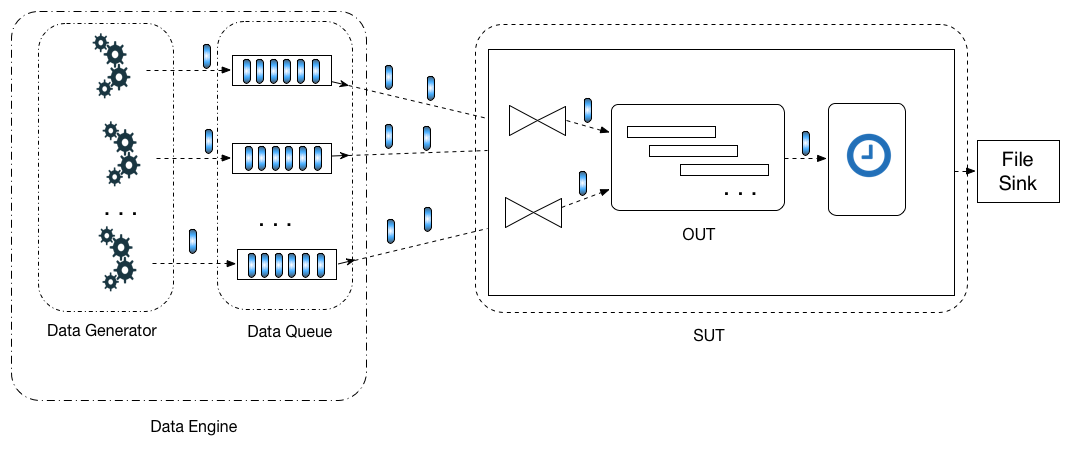
\includegraphics[width=1\textwidth]{eps/system_design}
\caption{Design of benchmark system.}
\label{fig_design}
\end{figure*}

\subsection{Use case}
The use case for this benchmark is provided by \textit{ Rovio Entertainment}. It is known as a video game development company. To get higher customer satisfaction, it is mandatory to analyse the game usage statistics. For example, company releases a new feature for a particular video game. It is essential to have a quick overview of customer's opinion by analysing the usage statistics. For that reason, Rovio uses stream data processing analytics rather than batch based periodic analysis.  In all use cases an event has following fields: event timestamp, key and value. 

\textbf{Windowed Aggregation}
Windowed aggregations are important part of the statistics analytics from the feed stream. One use case is computing the user average session time within windows. Each event has its geo ID, which indicate the location in which an event was generated. A use case includes partitioning the events by their ID and finding the average session time within windows. Here, the key field is geo location and value field is session time. Another use case is computing the average ads screening time within window for each geo location. 

\textbf{Windowed Join}
Joining several stream feeds based on key field within window is another general use case for user statistics analytics. One specific use case is joining two user statistics stream feed within window by geo field and calculating an event with higher session time and the difference between them. In this use case the key field would be geo location and value would be the session time. Another use case would be doing the same procedure with ads watch time. 


\subsection{Key Performance Indicators}
The Key Performance Indicators ( KPIs) for this benchmark are latency and throughput. The throughput indicator is related with SUT, on the other hand, the latency is associated with OUT. 


%To measure the performance of a system, we connected max $16$ data generators to system under test with order of $1$,$2$,$4$,$8$ and $16$ as increasing further does not increase the overall throughput significantly. We call the tests with related workloads as $1x$, $2x$, $4x$, $8x$ and $16x$. Moreover, the configuration of each data generator must be the same. Configuration includes parameters such as overall input size, generation speed, socket port and etc. Equation \ref{eq_2} defines this formally.
%
%\begin{equation}
%  \begin{gathered}
% \textbf{Let} \ d_{i}^{c_{i}} \in  D\\
%  \textbf{then}, |D| \gets S \\
%  \textbf{and} \ c_{1} = c_{2} \ ... = c_{n}, \forall n \in S = {1,2,4,8,16}
%  \end{gathered}\label{eq_2}
%\end{equation}


\subsubsection{Throughput}
\textit{Definition.  Let $c_{i} \in C$ be a configuration for a Data Engine, $d_{i} \in D$,  $c_{i}^{sp}$ be the data generation speed configuration which can be sustained by SUT. If  $\exists c_{i} \in C$ such that $c_{1} = c_{2}... = c_{i}$ and  $T = \sum_{i}c_{i}^{s}$ is maximum, $\forall c_{i} \in C, \forall i \in \{1,2,3 ... |C|\}$, then $T$ is a maximum sustainable throughput of SUT.}

Throughput of a system is calculated as summing the throughout of each Data Engine  because the SUT is expected to pull the data from all Data Queue subcomponent of Data Engine approximately with same rate. We restricted the configuration of all Data Engines to be the same, to ease calculating the maximum sustainable throughput. It is crucial to note that the maximum sustainable throughput is not the same as maximum throughput of Data Engine but the one for SUT. 

To examine the system's sustainability with a given throughput, we divide the queue used in Data Queue subcomponent into three parts: $c^{a}$ , $c^{b}$ and $c^{n}$. The Figure \ref{fig_queue}, shows the example partitioning of queue. If the size of the queue is less than or equal to $c^{a}$ then this is acceptable and means, the SUT can sustain the given throughput. If the queue size is less than or equal to $c^{b}$ on the other hand, the SUT cannot sustain the given data rate but we can tolerate it for some time, in case the increase in queue size is an outcome of back-pressure. However, if the queue size is bigger than the $c^{b}$ then the SUT cannot sustain the given throughput and there is no need to do benchmarks with particular data rate.

The semantics behind  examination of SUT's sustainability with a given throughput must be clear. Moreover, it should support the system specific behaviours like back-pressure. Algorithm \ref{alg_sustainable} show an algorithm to check if the  SUT can sustain  the given throughput of a single Data Engine. It gets the configuration $c$ of Data Engine as an input. After firing the Data Engine with configuration $c$, in line $3$, it is put to $idle$ position, meaning no data is generated until the SUT makes its first data pull request from Data Queue subcomponent. $c^{input}$ is the input count that must be generated in particular Data Engine.
 In lines $10-11$ the events are generated with speed $c^{sp}$ in Data Generator subcomponent of Data Engine component and put into the queue of Data Queue subcomponent. We check the queue size periodically, once per $c^{a}$ element and not for each iteration. The first reason is that the data pull rate of stream data processing engine is not steady and therefore checking the queue size with little delays makes more sense. The second reason is that, $c^{a}$ can be thought of the $confidence limit$ as shown in Figure \ref{fig_queue}. While checking the queue size there are three possibilities. The first is (lines $13-15$), the size is bigger than $c^{b}$, the back-pressure limit. In this case, the Data Engine is stopped and the $false$ is returned meaning the SUT is not sustainable with given throughput. The second is (lines $16-18$), queue size is less than $c^{a}$, the acceptable queue size. In this case, we set back-pressure counter to zero, in case there was one and continue generating data. The third is (lines $19-23$), the size   of queue is within boundaries of $c^{a}$ and $c^{b}$. In this case, we can tolerate the SUT for at most $\frac{c^{b}}{c^{a}}$ times. If the system can pull the data in queue and set the size of queue within \textit{confidence} boundaries ($c^{a}$) in a given period, then it continues, else, the application returns $false$ meaning, the SUT cannot sustain the given throughput. 

\begin{algorithm}
    \SetKwInOut{Input}{Input}
    \SetKwInOut{Output}{Output}

    \underline{function isSustainable} $(c)$\;
    \Input{ $c$ is configuration of Data Engine}
    \Output{return $true$ if is sustainable, $false$ otherwise}
    Fire Data Engines with configuration $c$. \\
    $c^{st} \gets idle$  \tcp*{wait for SUT to pull data}
  \While{There is no pull request from SUT}{
    wait \\ 
   }    
       $c^{st} \gets active$ \tcp*{start generating data}
       $bp\_index \gets 0$ \tcp*{initialize back-pressure index}
       \For{$i \gets 0; i < c^{input}; i++$}{
       Generate $e_{i} \in E$ with speed $c^{sp}$\\
       queue.put($e_{i}$) \tcp*{put  generated event to queue}
        \tcc{check the queue once per $c^{a}$ elements}
        \uIf{i \% $c^{a} == 0$}   { 
               \uIf{ $queue.size > c^{b}$  }   { 
              		Stop Data Engine \\
		         return $false$
               }
               \uElseIf{  $queue.size < c^{a}$ }{
               $bp\_index \gets 0$ \tcp*{ no back-pressure} 
               $continue$ \tcp*{SUT can sustain so far} 
               }
               \uElse{ 
                \tcc{ Tolerate for back-pressure}
                  $bp\_index \gets bp\_index +1$ \\
                     \uIf{$bp\_index == \frac{c^{b}}{c^{a}}$}{
                       \tcc{ This is not back-pressure}
                        Stop Data Engine \\
		         return $false$  
                     }
               }
        }
       }
    \caption{Throughput sustainability test of single data engine}
    \label{alg_sustainable}
\end{algorithm}

\textit{Definition.  Let $c_{i} \in C$ be a configuration for a Data Engine, $c_{i}^{dr}$ be a data generation rate of particular Data Generator, $d_{i} \in D$ and $n$ be the number of Data Engines being $n = |D|$.  The SUT is sustainable with given throughput $n * c_{dr}$,  $iff$ $isSustainable(c_{i})  == true$ $\forall$ $i \in \{1,2,3,...n\}$}

The above definition states that the SUT is sustainable with a given data generation rate iff, it can sustain all Data Engines at the same time. If one of the Data Engines cannot be sustained, then SUT is said is not sustainable with a given data generation rate. 


\subsubsection{Latency}
\label{sec_latency}
Latency is another KPI for this benchmark and defining the latency needs clear semantics. There are several points that needs to be clarified: \textit{i)} the aggregation or join of timestamp fields of tuples and \textit{ii)} clear boundaries (start and end timestamp) of latency.

The first point is the aggregation or join of tuples with timestamp fields. While the use case provides the semantics for aggregating or joining the tuples' $value$ fields, the one for timestamp field is unclear. For example, in windowed aggregation operator, which calculates the average of elements' $value$ field, the aggregation semantics with tuples' timestamp field is unclear.  The Equation \ref{eq_1} addresses this issue. Let $t[k]$ and $t'[k]$ denote the timestamp field for tuples $t$ and $t'$ respectively,  $\equiv$ be an operator checking for the type and $TS$ be tuple field of type timestamp. Here, $f_{s}$ is an stateful operator which takes a set of tuples $t \in T$ and converts it to tuple $t'$. Then there exists $k$ and $m$ such that the respective fields of input and output tuples have the same type being timestamp and the output tuple's timestamp is calculated taking maximum among input tuples. Here input and output tuples are associated with operator $f_{s}$ and not with the SUT.

To calculate the latency, it is crucial to have clear boundaries of when to start and stop the stopwatch for each tuple. Equation \ref{eq_2} defines the basic semantics behind this. This is basically a follow-up for Equation \ref{eq_1}. Let $t_{i} \in I$ be a tuple in input set and $t_{o} \in O$ be a tuple in output set. The latency is associated with output tuples. So, the latency of tuple $t_{o}$ is calculated by extracting the $t_{o}[m]$, the timestamps field from current time. The calculation of output tuples' timestamp field is shown in Equation \ref{eq_1}. 


\begin{equation}
  \begin{gathered}
\textbf{Let} f_{s}:\{t| t\in T \} \to t'  , \\
  \textbf{then}, \exists k,m \ s.t. \ t[k]  \equiv t'[m] \equiv \ TS \ \forall t \in T\\
  \textbf{and} \ t'[m] \gets \argmax\{t[k] \ | \ t \in T\}  
    \end{gathered}
      \label{eq_1} 
  \end{equation}

   \begin{equation}
     \begin{gathered}
  \textbf{Let} \ t_{i} \in I , t_{o} \in O \\
\textbf{then} \ Latency_{ \ t_{o}} = time_{now} -  t_{o}[m] \\
s.t. \ f_{s}:\{t_{i} \ | t_{i} \in I \} \to \{t_{o} \ | t_{o} \in O \} \\
\textbf{and} \ t_{o}[m] \equiv TS
  \end{gathered}
  \label{eq_2} 
\end{equation}



\begin{figure}[h]
\centering
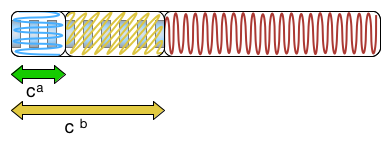
\includegraphics[width=0.7\textwidth]{eps/queue}
\caption{Basic intuition behind \textit{back-pressure-compatible queue}}
\label{fig_queue}
\end{figure}
